\documentclass[a4paper, 12pt]{article}
% math symbols
\usepackage{amssymb}
\usepackage{amsmath}
\usepackage{mathrsfs}
\usepackage{mathseries}


\usepackage[margin = 2cm]{geometry}

\tolerance = 1000
\emergencystretch = 0.74cm



\pagestyle{empty}
\parindent = 0mm

\renewcommand{\coursetitle}{DM/ML}
\setcounter{curtask}{1}

\setmathstyle{Апрель 23}{Теория информации}{2 курс}


\begin{document}

\libproblem{inf-theory}{shannon-fano}
\libproblem{inf-theory}{ariphmetic-balance}
\libproblem{inf-theory}{shannon-fano-opt}
\libproblem{inf-theory}{information-markov}
\libproblem{inf-theory}{stone-lift}

\begin{definition*}
    Определим общую информацию трёх случайных величин:
    $$
        I(\alpha : \beta : \gamma) \coloneqq I(\alpha : \beta) - I(\alpha : \beta \mid \gamma).
    $$

    Соотношения на информационные величины имеют удобную геометрическую интерпретацию. При помощи диаграмм
    Эйлера можно сопоставить площади каждой из получившихся замкнутых области некоторую информационную
    величину. В частности, прощать каждого круга соответствует энтропии указанной случайной величины.

    \begin{center}
        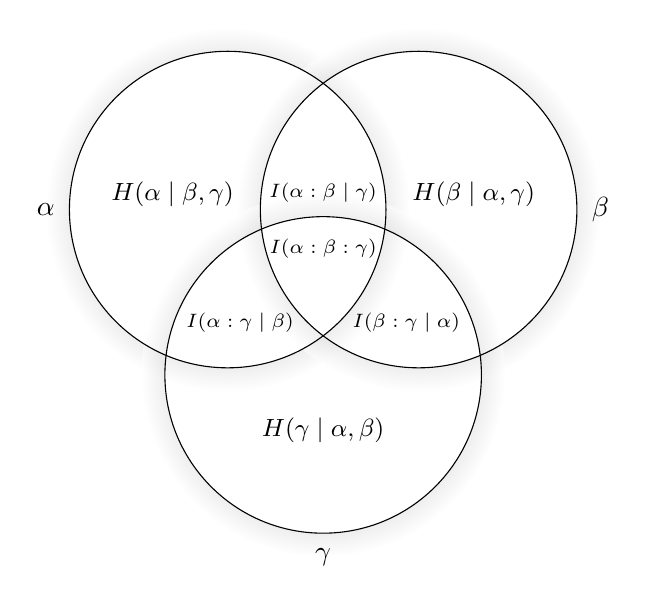
\begin{tikzpicture}
            \def\r{2.01}
            \def\R{1.4}

            \foreach \a in {150, 30, -90}{
                \shade[inner color = black, outer color = white, even odd rule, opacity = 0.5] (\a:\R)
                    circle (\r + 0.3) circle (\r);
            }
            
            \draw (150:\R) circle (\r) node[shift = {(-\r - 0.3, 0)}] {$\alpha$};
            \draw (30:\R) circle (\r) node[shift = {(\r + 0.3, 0)}] {$\beta$};
            \draw (-90:\R) circle (\r) node[shift = {(0, -\r - 0.3)}] {$\gamma$};

            \node[shift = {(-0.7, 0.2)}] at (150:\R) {\small $H(\alpha \mid \beta, \gamma)$};
            \node[shift = {(0.7, 0.2)}] at (30:\R) {\small $H(\beta \mid \alpha, \gamma)$};
            \node[shift = {(0, -0.7)}] at (-90:\R) {\small $H(\gamma \mid \alpha, \beta)$};

            \node at (90:0.65 * \R) {\scriptsize $I(\alpha : \beta \mid \gamma)$};
            \node at (-35:0.92 * \R) {\scriptsize $I(\beta : \gamma \mid \alpha)$};
            \node at (215:0.92 * \R) {\scriptsize $I(\alpha : \gamma \mid \beta)$};

            \node at (0, 0.2) {\scriptsize $I(\alpha : \beta : \gamma)$};
        \end{tikzpicture}
    \end{center}    
\end{definition*}

\libproblem{inf-theory}{negative-inf}

\begin{definition*}
    \deftext{Коммуникационный протокол} для функции $f: X \times Y \to Z$~--- это корневое двоичное
    дерево, которое описывает совместное вычисление Алисой и Бобом функции $f$. В этом дереве каждая
    внутренняя вершина $v$ помечена меткой $a$ или $b$, означающей очередь хода Алисы или Боба
    соответственно. Для каждой вершины, помеченной $a$, определена функция $g_v: X \to \{0, 1\}$, которая
    говорит Алисе, какой бит нужно послать, если вычисление находится в этой вершине. Аналогично, для
    каждой вершины $v$ с пометкой $b$ определена функция $h_v: Y \to \{0, 1\}$, которая определяет бит,
    который Боб должен отослать в этой вершине. Каждая внутренняя вершина имеет двух потомков, ребро к
    первому потомку помечено $0$, а ребро ко второму потомку помечено $1$. Каждый лист помечен значением
    из множества $Z$.

    Каждая пара входов $(x, y)$ определяет путь от корня до листа в описанном двоичном дереве
    естественным обрзом. Будем говорить, что коммуникационный протокол вычисляет функцию $f$, если для
    всех пар $(x, y) \in X \times Y$, этот путь заканчивается в листе с пометкой $f(x, y)$.

    \deftext{Коммуникационной сложностью} функции $f$ назовем наименьшую глубину протокола, вычисляющего
    функцию $f$, и будем ее обозначать $D(f)$.
\end{definition*}

\libproblem{cc}{basic-lower}

\breakline

\libproblem{inf-theory}{injective-code}


\end{document}



%%% Local Variables:
%%% mode: latex
%%% TeX-master: t
%%% End:
